\section{Python Class}

Using all of our knowledge of matrices and relations, we can create a class that can be used to determine the properties of a relation set. This class can be used to determine the properties of a relation set by using the matrix. 

I will use the following relation set as an example: \\

$R = \{(\emptyset ,\{a\}),(\emptyset,\{b\}),(\emptyset,\{a,b\}),(\{ a\} ,\{ b\}),(\{a\},\{a,b\}),(\{b\},\{a,b\})\}$ \\


The class is shown below:
\definecolor{mygreen}{rgb}{0,0.6,0}
\definecolor{mygray}{rgb}{0.5,0.5,0.5}
\definecolor{mymauve}{rgb}{0.58,0,0.82}

\lstset{ %
  backgroundcolor=\color{white},   % choose the background color
  basicstyle=\footnotesize,        % size of fonts used for the code
  breaklines=true,                 % automatic line breaking only at whitespace
  captionpos=b,                    % sets the caption-position to bottom
  commentstyle=\color{mygreen},    % comment style
  escapeinside={\%*}{*)},          % if you want to add LaTeX within your code
  keywordstyle=\color{purple},       % keyword style
  stringstyle=\color{mymauve},     % string literal style
}

\begin{lstlisting}[language=Python]
    import numpy as np

    class Relations():
        def __init__(self, s, R):
            self.s = s
            self.R = R
            self.M = np.zeros((len(s), len(s)))
            for i in R:
                self.M[i[0]-1][i[1]-1] = 1
    
        def returnMatrix(self):
            return self.M
    
        def isReflexive(self):
            for i in range(len(self.M)):
                if self.M[i][i] == 0:
                    return False
            return True
    
        def isIrreflexive(self):
            return not self.isReflexive()
    
        def isSymmetric(self):
            T = self.M.transpose()
            if np.array_equal(T, self.M):
                return True
            return False
    
        def isAntisymmetric(self):
            if self.isSymmetric():
                return False
            return True
    
        def isTransitive(self):
            M = self.M
            Msquare = np.dot(M, M)
            bFoundOne = False
            bFoundTwo = False
            # if only two elements are in the relation, then it is transitive (We cannot prove that R is not transitive. Such a proof actually has a special name: it is vacuously true that R is transitive.)
            if len(self.R) == 2:
                return True
    
            for i in range(len(Msquare)):
                for j in range(len(Msquare)):
                    if Msquare[i][j] == 1:
                        bFoundOne = True
                    if Msquare[j][i] == 2:
                        bFoundTwo = True
                if bFoundOne and bFoundTwo:
                    return True
            return False
    
        def isTrichotomy(self):
            #every pair of nodes has one and only one edge between them.        
            # get all the edges 
            edges = self.R
            # make sure that there are no duplicate edges
            for i in range(len(edges)):
                for j in range(len(edges)):
                    if edges[i][0] == edges[j][1] and edges[i][1] == edges[j][0]:
                        return False
            # make sure that there are no edges that are not in the relation                    
            for i in range(len(self.M)):
                for j in range(len(self.M)):
                    if self.M[i][j] == 0:
                        for k in range(len(edges)):
                            if edges[k][0] == i+1 and edges[k][1] == j+1:
                                return False
                    
            # each node can only have two edges
            for i in range(len(self.M)):
                count = 0
                for j in range(len(self.M)):
                    if self.M[i][j] == 1:
                        count += 1
                if count > 2:
                    return False
                          
            # must be asymmetric
            if self.isSymmetric():
                return False
                
            return True
    
        def EquivalenceRelation(self):
            if self.isReflexive() and self.isSymmetric() and self.isTransitive():
                return True
            return False
    
        def WeakPartialOrder(self):
            if self.isReflexive() and self.isTransitive() and self.isAntisymmetric():
                return True
            return False
    
        def StrictPartialOrder(self):
            if self.isTransitive() and self.isAntisymmetric() and self.isIrreflexive():
                return True
            return False
    
        def WeakTotalOrder(self):
            if self.isReflexive() and self.isTransitive() and self.isTrichotomy():
                return True
            return False
    
        def StrictTotalOrder(self):
            if self.isTransitive() and self.isTrichotomy() and self.isIrreflexive():
                return True
            return False
    
        def StrictEquivalenceRelation(self):
            if self.EquivalenceRelation() and self.isIrreflexive():
                return True
            return False
    
        def printPropertiesOfRelation(self):
            # print only the properties that are true
            if self.isReflexive():
                print("Reflexive")
            if self.isIrreflexive():
                print("Irreflexive")
            if self.isSymmetric():
                print("Symmetric")
            if self.isAntisymmetric():
                print("Antisymmetric")
            if self.isTransitive():
                print("Transitive")
            if self.isTrichotomy():
                print("Trichotomy")
            if self.EquivalenceRelation():
                print("Equivalence Relation")
            if self.StrictEquivalenceRelation():
                print("Strict Equivalence Relation")
            if self.WeakPartialOrder():
                print("Weak Partial Order")
            if self.StrictPartialOrder():
                print("Strict Partial Order")
            if self.WeakTotalOrder():
                print("Weak Total Order")
            if self.StrictTotalOrder():
                print("Strict Total Order")
    
    # Using set
    #s = {0,a,b,ab}
    #R = {(0,{a}),(0,{b}),(0,{a,b}),({a},{b}),({a},{a,b}),({b},{a,b})}
    
    # since our class uses numerical values, we need to convert the set to a list of numbers and tuples of ordered pairs
    s = [1, 2, 3,4]
    #    0  a  b  ab
    R = [(1, 2), (1, 3), (1, 4), (2, 3), (2, 4), (3, 4)]
    r1 = Relations(s, R)
    r1.printPropertiesOfRelation()
    
    # std output is:
    #   Irreflexive
    #   Antisymmetric
    #   Transitive
    #   Strict Partial Order
    
\end{lstlisting}

Graphing the relation as a matrix

$R = \begin{bmatrix}
0 & 1 & 1 & 1 \\
0 & 0 & 1 & 1 \\
0 & 0 & 0 & 1 \\
0 & 0 & 0 & 0
\end{bmatrix}$ \\


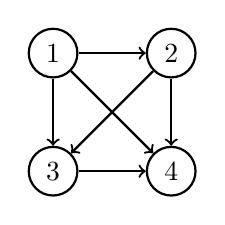
\begin{tikzpicture}[node distance={15mm}, thick, main/.style = {draw, circle}]
    \node[main] (1) {$1$}; 
    \node[main, right of=1] (2) {$2$};
    \node[main, below of=1] (3) {$3$};
    \node[main, below of=2] (4) {$4$};    
    \draw[->] (1) -- (2);
    \draw[->] (1) -- (3);
    \draw[->] (1) -- (4);
    \draw[->] (2) -- (3);
    \draw[->] (2) -- (4);
    \draw[->] (3) -- (4);
\end{tikzpicture} \\

 





\textbf{You may get the code from my GitHub Gist here.} \\

I hope this helps. \\

\href{https://gist.github.com/adgsenpai/4d8b24def8ffdcf82cc1cf43d8d89808}{Source Code}
